% ERD (Entity Relationship Diagram) - Sistem Informasi Usaha Bagan
% Dibuat dengan TikZ, kertas A3 landscape. Mencerminkan tabel database
% (model Django yang aktif). PK = primary key, FK = foreign key.
\documentclass[11pt]{article}
\usepackage[a3paper,landscape,margin=1cm]{geometry}
\usepackage[T1]{fontenc}
\usepackage[utf8]{inputenc}
\usepackage{tikz}
\usepackage{adjustbox}
\usetikzlibrary{arrows.meta,calc,shapes.multipart,positioning,fit}
\pagestyle{empty}

\tikzset{
  tbl/.style={draw=teal!60!black, rectangle split, rectangle split parts=2,
              font=\scriptsize, align=left, fill=teal!5, inner sep=3pt,
              rectangle split draw splits=true},
  rel/.style={thick, teal!55!black},
  one/.style={font=\footnotesize\bfseries, teal!45!black, inner sep=2pt},
  many/.style={font=\footnotesize\bfseries, teal!45!black, inner sep=2pt},
  % tabel & relasi nonaktif (sisa modul mobile/REST) -> diredupkan
  deadtbl/.style={draw=gray!55, rectangle split, rectangle split parts=2,
                  font=\scriptsize, align=left, fill=gray!8, inner sep=3pt,
                  rectangle split draw splits=true, text=black!65},
  deadrel/.style={thick, gray!50, dashed},
}
\newcommand{\PK}{\textbf{\underline{PK}}\,}
\newcommand{\FK}{\textit{FK}\,}

\begin{document}
\begin{adjustbox}{max width=\textwidth, max totalheight=\textheight, center}
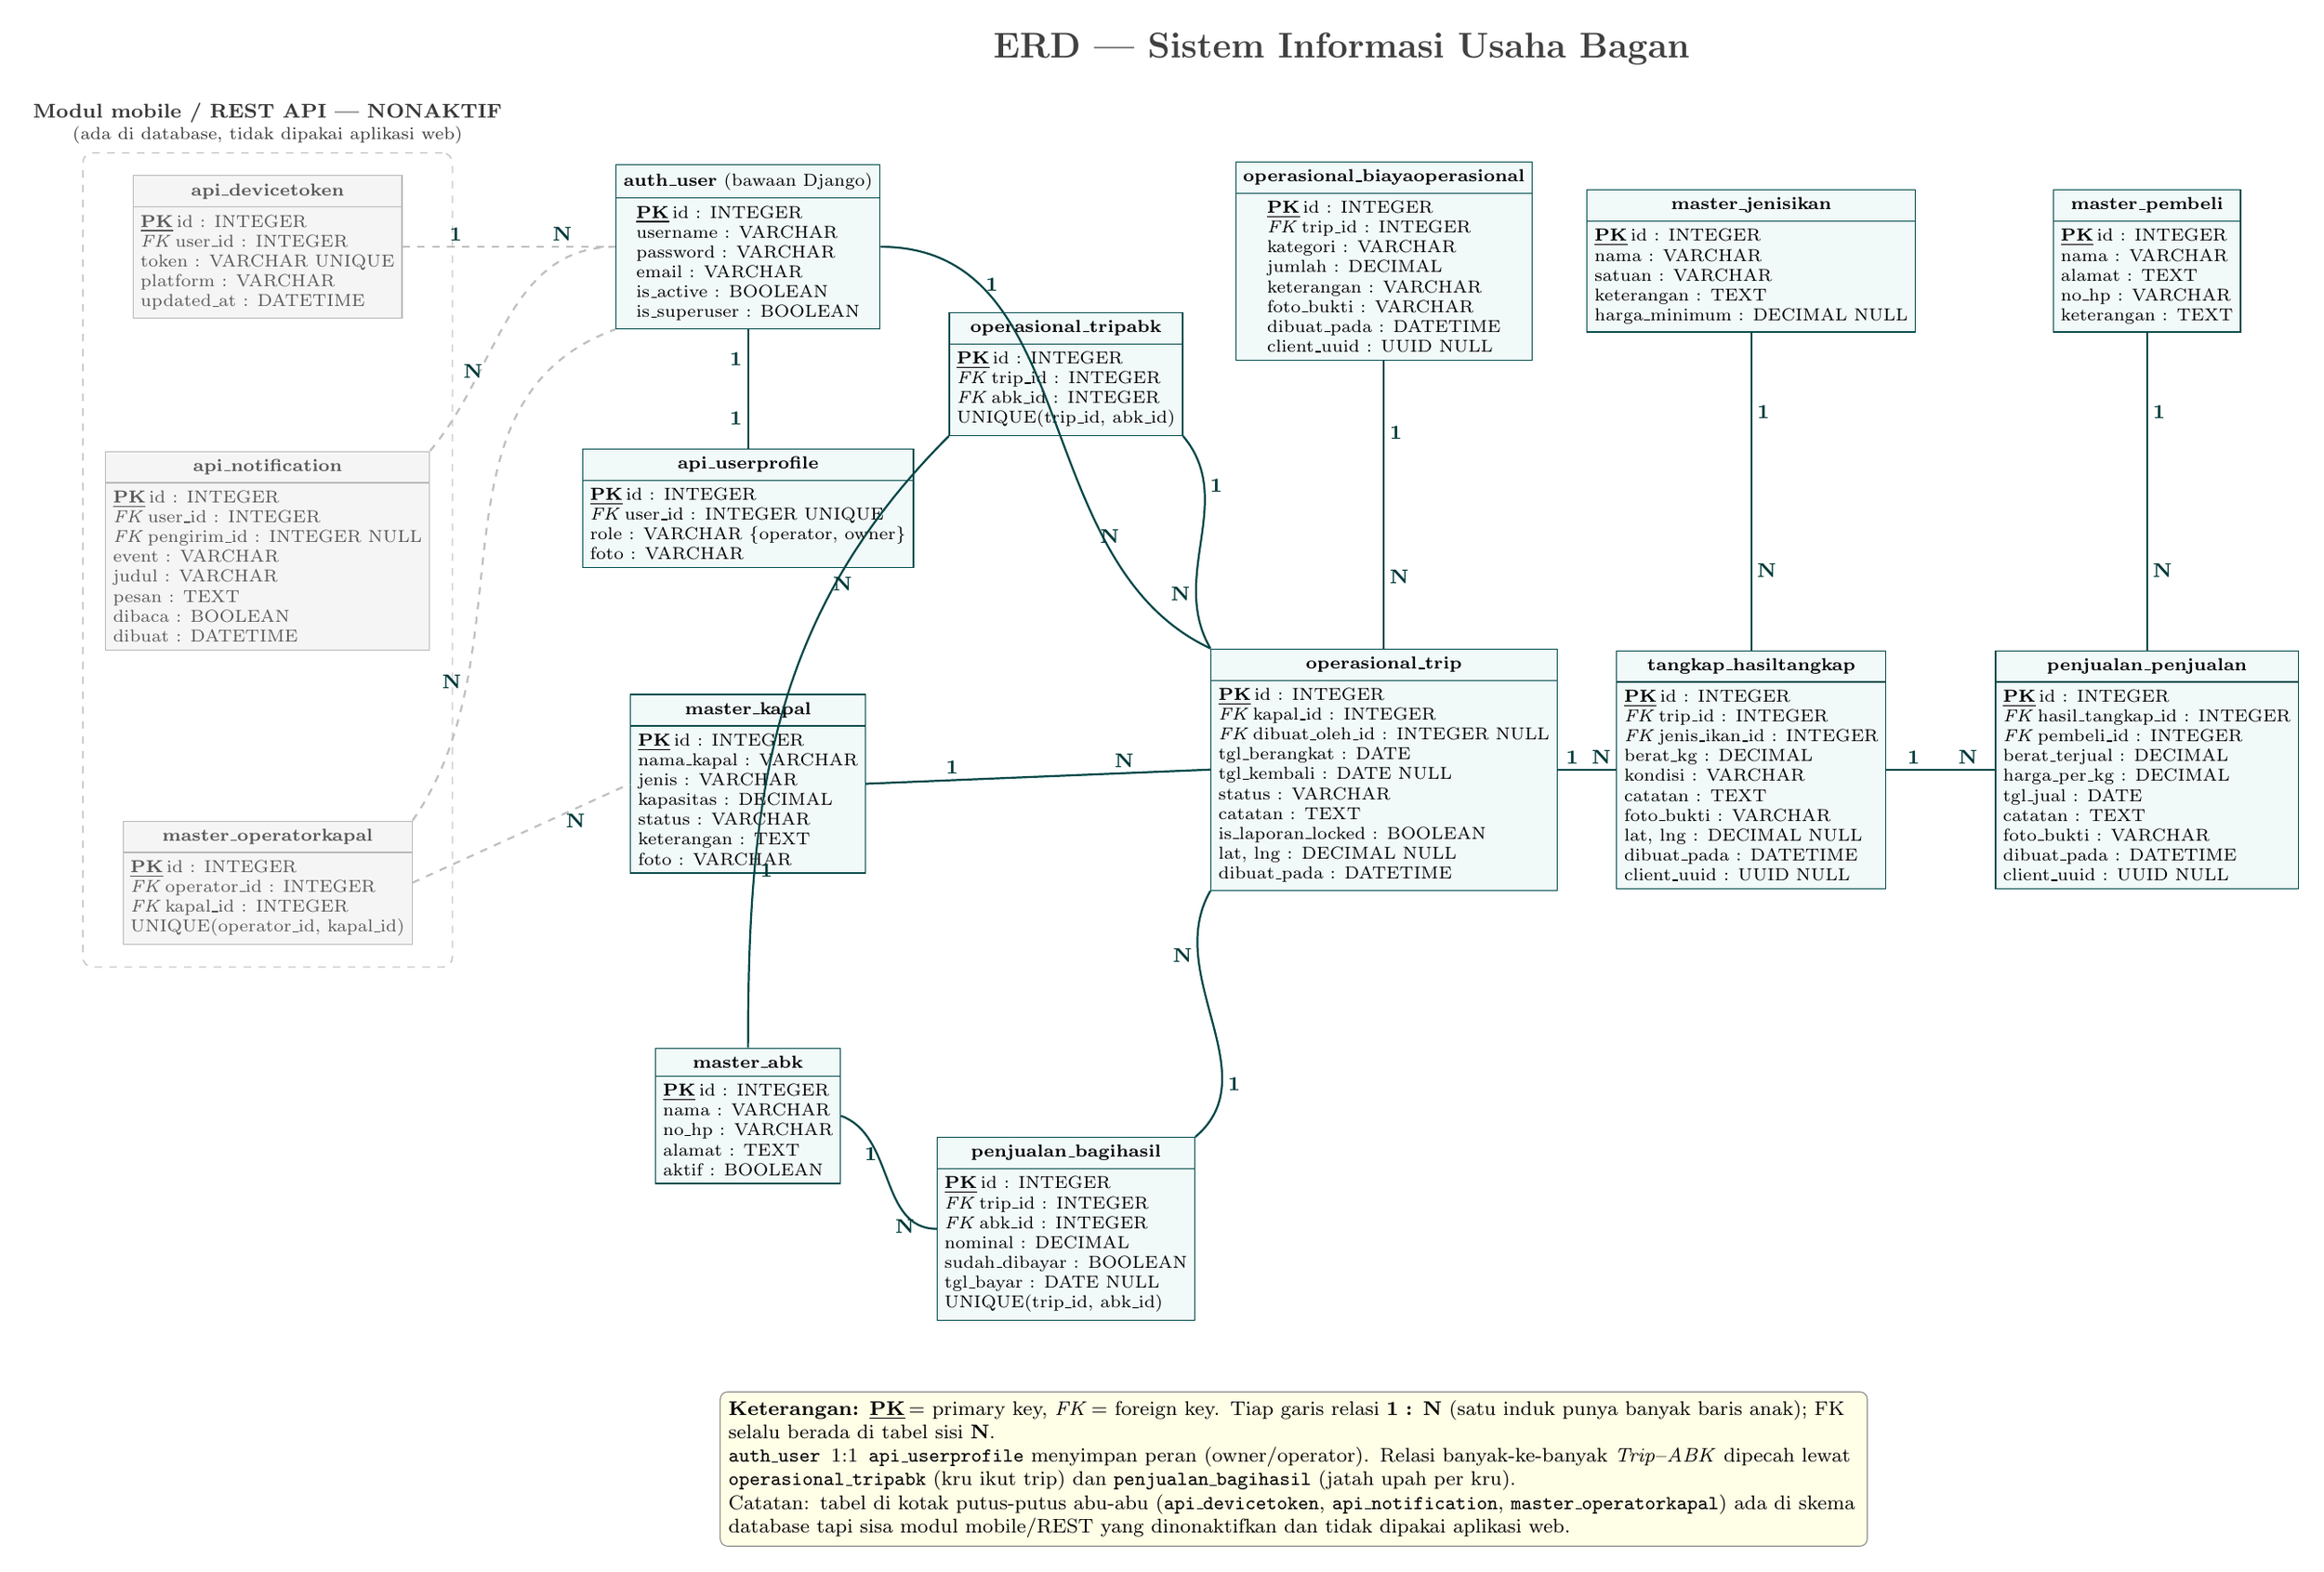
\begin{tikzpicture}[every node/.style={transform shape}]

\node[font=\Large\bfseries, black!75] at (10,15.8) {ERD — Sistem Informasi Usaha Bagan};

% =================== TABEL ===================
\node[tbl] (user) at (1.6,13) {\textbf{auth\_user} \scriptsize(bawaan Django)
  \nodepart{two}\PK id : INTEGER\\ username : VARCHAR\\ password : VARCHAR\\ email : VARCHAR\\ is\_active : BOOLEAN\\ is\_superuser : BOOLEAN};

\node[tbl] (profile) at (1.6,9.3) {\textbf{api\_userprofile}
  \nodepart{two}\PK id : INTEGER\\ \FK user\_id : INTEGER \scriptsize UNIQUE\\ role : VARCHAR \{operator, owner\}\\ foto : VARCHAR};

\node[tbl] (kapal) at (1.6,5.4) {\textbf{master\_kapal}
  \nodepart{two}\PK id : INTEGER\\ nama\_kapal : VARCHAR\\ jenis : VARCHAR\\ kapasitas : DECIMAL\\ status : VARCHAR\\ keterangan : TEXT\\ foto : VARCHAR};

\node[tbl] (abk) at (1.6,0.7) {\textbf{master\_abk}
  \nodepart{two}\PK id : INTEGER\\ nama : VARCHAR\\ no\_hp : VARCHAR\\ alamat : TEXT\\ aktif : BOOLEAN};

\node[tbl] (tripabk) at (6.1,11.2) {\textbf{operasional\_tripabk}
  \nodepart{two}\PK id : INTEGER\\ \FK trip\_id : INTEGER\\ \FK abk\_id : INTEGER\\ \scriptsize UNIQUE(trip\_id, abk\_id)};

\node[tbl] (bagihasil) at (6.1,-0.9) {\textbf{penjualan\_bagihasil}
  \nodepart{two}\PK id : INTEGER\\ \FK trip\_id : INTEGER\\ \FK abk\_id : INTEGER\\ nominal : DECIMAL\\ sudah\_dibayar : BOOLEAN\\ tgl\_bayar : DATE \scriptsize NULL\\ \scriptsize UNIQUE(trip\_id, abk\_id)};

\node[tbl] (trip) at (10.6,5.6) {\textbf{operasional\_trip}
  \nodepart{two}\PK id : INTEGER\\ \FK kapal\_id : INTEGER\\ \FK dibuat\_oleh\_id : INTEGER \scriptsize NULL\\ tgl\_berangkat : DATE\\ tgl\_kembali : DATE \scriptsize NULL\\ status : VARCHAR\\ catatan : TEXT\\ is\_laporan\_locked : BOOLEAN\\ lat, lng : DECIMAL \scriptsize NULL\\ dibuat\_pada : DATETIME};

\node[tbl] (biaya) at (10.6,12.8) {\textbf{operasional\_biayaoperasional}
  \nodepart{two}\PK id : INTEGER\\ \FK trip\_id : INTEGER\\ kategori : VARCHAR\\ jumlah : DECIMAL\\ keterangan : VARCHAR\\ foto\_bukti : VARCHAR\\ dibuat\_pada : DATETIME\\ client\_uuid : UUID \scriptsize NULL};

\node[tbl] (tangkap) at (15.8,5.6) {\textbf{tangkap\_hasiltangkap}
  \nodepart{two}\PK id : INTEGER\\ \FK trip\_id : INTEGER\\ \FK jenis\_ikan\_id : INTEGER\\ berat\_kg : DECIMAL\\ kondisi : VARCHAR\\ catatan : TEXT\\ foto\_bukti : VARCHAR\\ lat, lng : DECIMAL \scriptsize NULL\\ dibuat\_pada : DATETIME\\ client\_uuid : UUID \scriptsize NULL};

\node[tbl] (jenisikan) at (15.8,12.8) {\textbf{master\_jenisikan}
  \nodepart{two}\PK id : INTEGER\\ nama : VARCHAR\\ satuan : VARCHAR\\ keterangan : TEXT\\ harga\_minimum : DECIMAL \scriptsize NULL};

\node[tbl] (penjualan) at (21.4,5.6) {\textbf{penjualan\_penjualan}
  \nodepart{two}\PK id : INTEGER\\ \FK hasil\_tangkap\_id : INTEGER\\ \FK pembeli\_id : INTEGER\\ berat\_terjual : DECIMAL\\ harga\_per\_kg : DECIMAL\\ tgl\_jual : DATE\\ catatan : TEXT\\ foto\_bukti : VARCHAR\\ dibuat\_pada : DATETIME\\ client\_uuid : UUID \scriptsize NULL};

\node[tbl] (pembeli) at (21.4,12.8) {\textbf{master\_pembeli}
  \nodepart{two}\PK id : INTEGER\\ nama : VARCHAR\\ alamat : TEXT\\ no\_hp : VARCHAR\\ keterangan : TEXT};

% =================== TABEL NONAKTIF (modul mobile/REST) ===================
\node[deadtbl] (devicetoken) at (-5.2,13.0) {\textbf{api\_devicetoken}
  \nodepart{two}\PK id : INTEGER\\ \FK user\_id : INTEGER\\ token : VARCHAR \scriptsize UNIQUE\\ platform : VARCHAR\\ updated\_at : DATETIME};

\node[deadtbl] (notification) at (-5.2,8.7) {\textbf{api\_notification}
  \nodepart{two}\PK id : INTEGER\\ \FK user\_id : INTEGER\\ \FK pengirim\_id : INTEGER \scriptsize NULL\\ event : VARCHAR\\ judul : VARCHAR\\ pesan : TEXT\\ dibaca : BOOLEAN\\ dibuat : DATETIME};

\node[deadtbl] (operatorkapal) at (-5.2,4.0) {\textbf{master\_operatorkapal}
  \nodepart{two}\PK id : INTEGER\\ \FK operator\_id : INTEGER\\ \FK kapal\_id : INTEGER\\ \scriptsize UNIQUE(operator\_id, kapal\_id)};

\node[draw=gray!55, dashed, rounded corners, inner sep=9pt, fill=none,
      fit=(devicetoken)(notification)(operatorkapal)] (deadbox) {};
\node[gray!45!black, font=\footnotesize\bfseries, align=center, anchor=south]
      at (deadbox.north) {Modul mobile / REST API — NONAKTIF\\[-1pt]
      \scriptsize\mdseries (ada di database, tidak dipakai aplikasi web)};

% relasi tabel nonaktif (semua mengarah ke auth_user / master_kapal)
\draw[deadrel] (devicetoken.east)   -- node[one,near start,above]{1} node[many,near end,above]{N} (user.west);
\draw[deadrel] (notification.north east) to[out=50,in=180] node[many,near start,above]{N} (user.west);
\draw[deadrel] (operatorkapal.east) -- node[many,near end,below]{N} (kapal.west);
\draw[deadrel] (operatorkapal.north east) to[out=55,in=200] node[many,near start,left]{N} (user.south west);

% =================== RELASI (1 : N) ===================
\draw[rel] (user.south) -- node[one,near start,left]{1} node[one,near end,left]{1} (profile.north);
\draw[rel] (user.east) to[out=0,in=155] node[one,near start,above]{1} node[many,near end,above]{N} (trip.north west);
\draw[rel] (kapal.east) -- node[one,near start,above]{1} node[many,near end,above]{N} (trip.west);
\draw[rel] (abk.north) to[out=90,in=-135] node[one,near start,right]{1} node[many,near end,below]{N} (tripabk.south west);
\draw[rel] (abk.east) to[out=-20,in=180] node[one,near start,below]{1} node[many,near end,below]{N} (bagihasil.west);
\draw[rel] (trip.north west) to[out=120,in=-50] node[one,near end,right]{1} node[many,near start,left]{N} (tripabk.south east);
\draw[rel] (trip.south west) to[out=-120,in=40] node[one,near end,right]{1} node[many,near start,left]{N} (bagihasil.north east);
\draw[rel] (trip.north) -- node[one,near end,right]{1} node[many,near start,right]{N} (biaya.south);
\draw[rel] (trip.east) -- node[one,near start,above]{1} node[many,near end,above]{N} (tangkap.west);
\draw[rel] (jenisikan.south) -- node[one,near start,right]{1} node[many,near end,right]{N} (tangkap.north);
\draw[rel] (tangkap.east) -- node[one,near start,above]{1} node[many,near end,above]{N} (penjualan.west);
\draw[rel] (pembeli.south) -- node[one,near start,right]{1} node[many,near end,right]{N} (penjualan.north);

% =================== LEGENDA ===================
\node[draw=black!45, rounded corners=3pt, align=left, font=\footnotesize,
      fill=yellow!10, text width=16cm, anchor=north west] at (1.2,-3.2)
  {\textbf{Keterangan:} \PK = primary key, \FK = foreign key. Tiap garis relasi \textbf{1 : N}
   (satu induk punya banyak baris anak); FK selalu berada di tabel sisi \textbf{N}.\\
   \texttt{auth\_user} \,1:1\, \texttt{api\_userprofile} menyimpan peran (owner/operator).
   Relasi banyak-ke-banyak \emph{Trip}–\emph{ABK} dipecah lewat \texttt{operasional\_tripabk}
   (kru ikut trip) dan \texttt{penjualan\_bagihasil} (jatah upah per kru).\\
   Catatan: tabel di kotak putus-putus abu-abu (\texttt{api\_devicetoken},
   \texttt{api\_notification}, \texttt{master\_operatorkapal}) ada di skema database
   tapi sisa modul mobile/REST yang dinonaktifkan dan tidak dipakai aplikasi web.};

\end{tikzpicture}%
\end{adjustbox}
\end{document}
